%<<echo=FALSE>>=
%OLD <- options(width=90)
%@
%<<echo=FALSE>>=
%options(OLD) 
%@

\documentclass{beamer}\usepackage[]{graphicx}\usepackage[]{color}
%% maxwidth is the original width if it is less than linewidth
%% otherwise use linewidth (to make sure the graphics do not exceed the margin)
\makeatletter
\def\maxwidth{ %
  \ifdim\Gin@nat@width>\linewidth
    \linewidth
  \else
    \Gin@nat@width
  \fi
}
\makeatother

\definecolor{fgcolor}{rgb}{0.102, 0.102, 0.102}
\newcommand{\hlnum}[1]{\textcolor[rgb]{0.2,0.2,0.2}{#1}}%
\newcommand{\hlstr}[1]{\textcolor[rgb]{0.2,0.2,0.2}{#1}}%
\newcommand{\hlcom}[1]{\textcolor[rgb]{0.302,0.302,0.302}{\textit{#1}}}%
\newcommand{\hlopt}[1]{\textcolor[rgb]{0.102,0.102,0.102}{#1}}%
\newcommand{\hlstd}[1]{\textcolor[rgb]{0.102,0.102,0.102}{#1}}%
\newcommand{\hlkwa}[1]{\textcolor[rgb]{0.102,0.102,0.102}{#1}}%
\newcommand{\hlkwb}[1]{\textcolor[rgb]{0.102,0.102,0.102}{#1}}%
\newcommand{\hlkwc}[1]{\textcolor[rgb]{0.2,0.2,0.2}{#1}}%
\newcommand{\hlkwd}[1]{\textcolor[rgb]{0.102,0.102,0.102}{\textbf{#1}}}%

\usepackage{framed}
\makeatletter
\newenvironment{kframe}{%
 \def\at@end@of@kframe{}%
 \ifinner\ifhmode%
  \def\at@end@of@kframe{\end{minipage}}%
  \begin{minipage}{\columnwidth}%
 \fi\fi%
 \def\FrameCommand##1{\hskip\@totalleftmargin \hskip-\fboxsep
 \colorbox{shadecolor}{##1}\hskip-\fboxsep
     % There is no \\@totalrightmargin, so:
     \hskip-\linewidth \hskip-\@totalleftmargin \hskip\columnwidth}%
 \MakeFramed {\advance\hsize-\width
   \@totalleftmargin\z@ \linewidth\hsize
   \@setminipage}}%
 {\par\unskip\endMakeFramed%
 \at@end@of@kframe}
\makeatother

\definecolor{shadecolor}{rgb}{.97, .97, .97}
\definecolor{messagecolor}{rgb}{0, 0, 0}
\definecolor{warningcolor}{rgb}{1, 0, 1}
\definecolor{errorcolor}{rgb}{1, 0, 0}
\newenvironment{knitrout}{}{} % an empty environment to be redefined in TeX

\usepackage{alltt}% regular slides (with pauses)
%\documentclass[handout]{beamer}% handout (no pauses)

%%%%%%%%%%%%%%%%%%%%%%%%%%%%%%%%%%%%%%%%%%%%%%%%%%%%%%%%%%%%%%%%%%%%%%%%%
%%%%%%% Change the lecture information here %%%%%%%%%%%%%%%%
\def\chapnum{Week \#5}
\title{STAT234: Lecture 5 - Hypothesis Testing}
\author{Kushal K. Dey}
\date{}
%%%%%%%%%%%%%%%%%%%%%%%%%%%%%%%%%%%%%%%%%%%%%%%%%%%%%%%%%%%%%%%%%%%%%%%%%

%%%%%% Start of suggested definitions and packages %%%%%%%%%%%%
%%%%%% Do not change unless you really know what you are doing %%%%%%%%%%
%%%%%%%%%%%%%%%%%%%%%%%%%%%%%%%%%%%%%%%%%%%%%%%%%%%%%%%%%%%%%%%%%%%%%%%%%

\usepackage{enumerate}
\usepackage{amsmath, bbm}
\usepackage[misc]{ifsym} % for the dice symbol \Cube{}
\usepackage[latin1]{inputenc}
\usepackage{hyperref}

%\usepackage{comment}
%\usepackage{pstricks}
%\usepackage{graphicx}
%\usepackage{booktabs}
%\usepackage{pgfpages}
%\pgfpagesuselayout{2 on 1}[a4paper,border shrink=3mm]
%\pgfpagesuselayout{4 on 1}[a4paper,landscape,border shrink=3mm

\usepackage{setspace}
\ifdefined\knitrout
  \renewenvironment{knitrout}{\begin{spacing}{0.75}\begin{tiny}}{\end{tiny}\end{spacing}}
\else
\fi

%%%%%%%%%%%%%%% Defined Shortcuts (macros) %%%%%%%%%%%%%
% parameters and statistics
\newcommand{\xbar}{\overline{x}}
\newcommand{\Xbar}{\overline{X}}
\newcommand{\ybar}{\overline{y}}
\newcommand{\Ybar}{\overline{Y}}
\newcommand{\dbar}{\overline{d}}
\newcommand{\Dbar}{\overline{D}}
\newcommand{\zbar}{\overline{z}}
\newcommand{\Zbar}{\overline{Z}}
\newcommand{\ehat}{\widehat{\epsilon}}
\newcommand{\yhat}{\widehat{y}}
\newcommand{\Yhat}{\widehat{Y}}
\newcommand{\betaa}{{\beta_0}}
\newcommand{\betab}{{\beta_1}}
\newcommand{\betac}{{\beta_2}}
\newcommand{\betad}{{\beta_3}}
\newcommand{\BETA}{{\boldsymbol\beta}}
\newcommand{\betahata}{\widehat{\beta_0}}
\newcommand{\betahatb}{\widehat{\beta_1}}
\newcommand{\betahatc}{\widehat{\beta_2}}
\newcommand{\betahatd}{\widehat{\beta_3}}
\newcommand{\bhat}{\widehat{b}}
\newcommand{\btilde}{\widetilde{b}}
\newcommand{\ahat}{\widehat{a}}
\newcommand{\atilde}{\widetilde{a}}
\newcommand{\rss}{\mathit{SSE}}
\newcommand{\sigmahat}{\widehat{\sigma}}
\newcommand{\betahat}{\widehat{\beta}}
\newcommand{\thetahat}{\widehat{\theta}}
\newcommand{\phat}{\widehat{p}}
\newcommand{\pihat}{\widehat{\pi}}
\newcommand{\muhat}{\widehat{\mu}}
% real numbers and integers
\newcommand{\reals}{\mathbbm{R}}
\newcommand{\integers}{\mathbbm{N}}
%distributions
\newcommand{\normal}{\textsf{Norm}}
\newcommand{\Bin}{\textsf{Binom}}
\newcommand{\Uni}{\textsf{Unif}}
\newcommand{\Poisson}{\textsf{Pois}}
\newcommand{\Exp}{\textsf{Exp}}
\newcommand{\Beta}{\textsf{Beta}}
\newcommand{\iid}{\stackrel{\mathrm{iid}}{\sim}}
% probability and expected value
\newcommand{\rv}{r.v.\ }
\newcommand{\prob}{{\rm P}}
\newcommand{\mean}{\mathrm{E}}
\newcommand{\var}{\mathrm{Var}}
\newcommand{\Var}{\mathrm{Var}}
\newcommand{\cov}{\mathrm{Cov}}
\newcommand{\corr}{\mathop{\mathrm{Corr}}}
% measures of spread
\newcommand{\IQR}{\textit{IQR}}
\newcommand{\SAD}{\textit{SAD}}
\newcommand{\MAD}{\textit{MAD}}
\newcommand{\SSD}{\textit{SSD}}
\newcommand{\MSD}{\textit{MSD}}
\newcommand{\RMSD}{\textit{RMSD}}
\newcommand{\MSE}{\textit{MSE}}
\newcommand{\MSR}{\textit{MSR}}
% formatting code and such
\providecommand{\variable}[1]{}
\renewcommand{\variable}[1]{{\color{green!50!black}\texttt{#1}}}
\providecommand{\function}[1]{}
\renewcommand{\function}[1]{{\color{purple!75!blue}\texttt{\StrSubstitute{#1}{()}{}()}}}
\providecommand{\option}[1]{}
\renewcommand{\option}[1]{{\color{brown!80!black}\texttt{#1}}}
\providecommand{\pkg}[1]{}
\renewcommand{\pkg}[1]{{\color{red!80!black}\texttt{#1}}}
\providecommand{\code}[1]{}
\renewcommand{\code}[1]{{\color{blue!80!black}\texttt{#1}}}

%%%%%%%%%
% Changed by Kushal K Dey, University of Chicago
%\providecommand{\file}[1]{}
%\renewcommand{\file}[1]{{\tt #1}}
\providecommand{\file}[1]{}
\renewcommand{\file}[1]{{\color{orange!80!black}\texttt{#1}}}
%\providecommand{\dataframe}[1]{}
%\renewcommand{\dataframe}[1]{{\color{blue!80!black}\texttt{#1}}}
\providecommand{\dataframe}[1]{}
\renewcommand{\dataframe}[1]{{\color{cyan!80!black}\texttt{#1}}}
%%%%%%%%%

% other
\def\Sum{\sum\nolimits}
\def\b#1{\fboxsep=0pt\colorbox{black}{\color{white}\Cube{#1}}}
\def\w#1{\Cube{#1}}
%%%%%%%%%%%% End of shortcuts (macros) ##############

%%%%%%%%% One way to hide answers until you want to show them %%%%%%%%%
\def\Hide#1#2{\ul{~~~\onslide<#1>{\alert{#2}}~~~}}
\def\hide#1#2{\ul{~~\onslide<#1>{\alert{#2}}~~}}
\def\hid#1#2{\onslide<#1>{\alert{#2}}}
% Choose the color of answers here too
\setbeamercolor{alerted text}{fg=darkgray} 
%\setbeamercolor{alerted text}{fg=black} 

%------Centered Page Number Setup ------
\defbeamertemplate{footline}{centered page number}
{%
  \hspace*{\fill}%
  %\usebeamercolor[fg]{page number in head/foot}%
  %\usebeamerfont{page number in head/foot}%
  \tiny \chapnum: Page \insertframenumber\, of \inserttotalframenumber%
  \hspace*{\fill}\vskip2pt%
}
%\setbeamertemplate{footline}{\hfill\insertframenumber/\inserttotalframenumber}
\setbeamertemplate{footline}[centered page number]
%--------------------------------

%\usetheme{Copenhagen}
\setbeamertemplate{navigation symbols}{}
\usepackage[english]{babel}
\def\ul{\underline}
\linespread{1.1}
% or whatever



%\parskip=0pt
\IfFileExists{upquote.sty}{\usepackage{upquote}}{}
\begin{document}%large

%<<setup, include=FALSE, cache=FALSE>>=
%options(replace.assign=TRUE,width=90, digits=4)
%opts_chunk$set(fig.path='figure/graphics-', cache.path='cache/graphics-', fig.align='center', fig.width=8, fig.height=4.5, fig.show='as.is', out.width='0.9\\linewidth', cache=FALSE, par=TRUE, size = 'tiny', tidy=TRUE, cache.extra=rand_seed)
%knit_hooks$set(par=function(before, options, envir){
%if (before && options$fig.show!='none') par(mar=c(4,4,.1,.1),cex.lab=.95,cex.axis=.9,mgp=c(2,.7,0),tcl=-.3)
%}, document = function(x) {
%  gsub('\\\\(begin|end)\\{kframe\\}', '', x)
%}, crop=hook_pdfcrop)
%@
%<<setup2, include=FALSE, cache=FALSE>>=
%knit_theme$set("print")
%@


%%%%%%%%%%%%%%%%%%%%%%%%%%%%%%%%%%%%%%%%%%%%%%%%%%%%%%%%%%%%%%%%%%%%%%%%%
%%%%%%%%%%%%%%%%%%%%%%%%%%%%%%%%%%%%%%%%%%%%%%%%%%%%%%%%%%%%%%%%%%%%%%%%%
%%%%%% End of suggested definitions and packages %%%%%%%%%%%%

%------------------------------------------------------------------
%------------------------------------------------------------------

%%%%%%%%%% Title frame (optional) %%%%%%%%%%%%%
\begin{frame}{}
\maketitle
\end{frame}
%%%%%%%%%%%%%%%%%%%%%%%%%%%%%%%%%%%%%%%%%%%%%%%

%%%%%%%%%%%%%% Begin slides here %%%%%%%%%%%%%%

%%%%%%%%%%%%%%%%%%%%%%%%%%%%%%%%%%%%%%%%%%%%%%%%%%%%%%%%%%%%
\begin{frame}[fragile]
%%%%%%%%%%%%%%%%%%%%%%%%%%%%%%%%%%%%%%%%%%%%%%%%%%%%%%%%%%%%

\begin{itemize}
\item Random Experiment- States, Events \pause
\item Random Variables - functions on states \pause
\item Probability - proportion of occurence under infinitely many trials \pause
\item Probability table for Random variable \pause
\item Expectation \pause
\item Variance \pause
\item Moment generating function:  \pause
\item Sums of random variables \pause
\item Expectation and variance of sums of random variables \pause
\item Sampling proportion  \pause
\item Generalization to continuous distribution \pause
\item Bernoulli, Binomial and Normal Distribution 
\end{itemize}

\end{frame}
%%%%%%%%%%%%%%%%%%%%%%%%%%%%%%%%%%%%%%%%%%%%%%%


%%%%%%%%%%%%%%%%%%%%%%%%%%%%%%%%%%%%%%%%%%%%%%%%%%%%%%%%%%%%
\begin{frame}[fragile]
%%%%%%%%%%%%%%%%%%%%%%%%%%%%%%%%%%%%%%%%%%%%%%%%%%%%%%%%%%%%

\Huge{\centering Where is the Statistics in all this?}

\end{frame}
%%%%%%%%%%%%%%%%%%%%%%%%%%%%%%%%%%%%%%%%%%%%%%%

%%%%%%%%%%%%%%%%%%%%%%%%%%%%%%%%%%%%%%%%%%%%%%%%%%%%%%%%%%%%
\begin{frame}[fragile]
%%%%%%%%%%%%%%%%%%%%%%%%%%%%%%%%%%%%%%%%%%%%%%%%%%%%%%%%%%%%

\Huge{\centering How can I use these concepts?}

\end{frame}
%%%%%%%%%%%%%%%%%%%%%%%%%%%%%%%%%%%%%%%%%%%%%%%

%%%%%%%%%%%%%%%%%%%%%%%%%%%%%%%%%%%%%%%%%%%%%%%%%%%%%%%%%%%%
\begin{frame}[fragile]
%%%%%%%%%%%%%%%%%%%%%%%%%%%%%%%%%%%%%%%%%%%%%%%%%%%%%%%%%%%%

\frametitle{A Romantic Experiment !}


\begin{center}
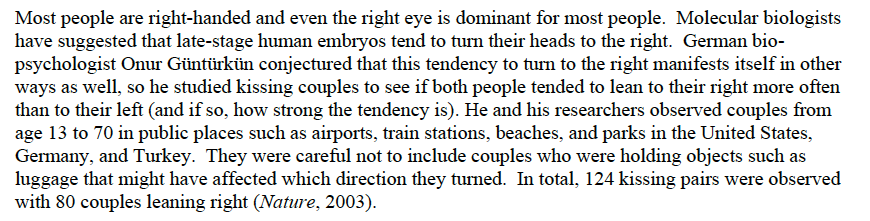
\includegraphics[width=11.5cm,height=5.3 cm]{KissingRight_StudyDescription.png}
\end{center}

\end{frame}
%%%%%%%%%%%%%%%%%%%%%%%%%%%%%%%%%%%%%%%%%%%%%%%

%%%%%%%%%%%%%%%%%%%%%%%%%%%%%%%%%%%%%%%%%%%%%%%%%%%%%%%%%%%%
\begin{frame}[fragile]
%%%%%%%%%%%%%%%%%%%%%%%%%%%%%%%%%%%%%%%%%%%%%%%%%%%%%%%%%%%%

\frametitle{View the data as random experiment}

Assume that the probability of leaning to right while kissing is $p$ \pause \newline

This means, if they had taken \textit{all possible couples} and recorded them kissing, 
and noted the proportion, it would have been $p$. \pause \newline

But thats damn difficult !! \pause \newline

Researchers however want to know about $p$, so they sample $124$ couples.

\end{frame}
%%%%%%%%%%%%%%%%%%%%%%%%%%%%%%%%%%%%%%%%%%%%%%%

%%%%%%%%%%%%%%%%%%%%%%%%%%%%%%%%%%%%%%%%%%%%%%%%%%%%%%%%%%%%
\begin{frame}[fragile]
%%%%%%%%%%%%%%%%%%%%%%%%%%%%%%%%%%%%%%%%%%%%%%%%%%%%%%%%%%%%

For each kissing couple, we define a random experiment, with two states \pause

$$ \mathcal{S} : \left \{ Kiss \; leaning \; right, Kiss \; not \; leaning \; right \right \} $$  \pause \newline

define a random variable $X$,

\begin{align}
X & = 1 \;\; Kiss \; leaning  \; right \\
  & = 0 \; \; Kiss \; not \; leaning \; right  \\
\end{align} \pause

$$ Pr \left [ X=1 \right ] : = Pr \left[ Kiss \; leaning \; right \right ] = p $$ \pause

\textbf{We do not know p !!} 

\end{frame}
%%%%%%%%%%%%%%%%%%%%%%%%%%%%%%%%%%%%%%%%%%%%%%%

%%%%%%%%%%%%%%%%%%%%%%%%%%%%%%%%%%%%%%%%%%%%%%%%%%%%%%%%%%%%
\begin{frame}[fragile]
%%%%%%%%%%%%%%%%%%%%%%%%%%%%%%%%%%%%%%%%%%%%%%%%%%%%%%%%%%%%

The researchers observed 124 couples. \pause \newline

This is same as saying, they observed realizations of $124$ random variables 
$X_1$, $X_2$, $\cdots$, $X_{124}$. \pause \newline

And they observed $80$ of them gave $1$ and the rest $48$ gave $0$. \pause \newline

What is $80 ?$

$$ \sum_{i=1}^{n} X_{i} = 80 $$
$$ \hat{p} = \frac{1}{n} \sum_{i=1}^{n} X_{i} = \frac{80}{124} = \frac{5}{8} $$

$\hat{p}$ is called the sampling proportion- here proportion of kissing right observed.

\end{frame}
%%%%%%%%%%%%%%%%%%%%%%%%%%%%%%%%%%%%%%%%%%%%%%%


%%%%%%%%%%%%%%%%%%%%%%%%%%%%%%%%%%%%%%%%%%%%%%%%%%%%%%%%%%%%
\begin{frame}[fragile]
%%%%%%%%%%%%%%%%%%%%%%%%%%%%%%%%%%%%%%%%%%%%%%%%%%%%%%%%%%%%

\frametitle{Hypothesis Testing}

\begin{itemize}
\item Choosing between two statements about a parameter. \pause
\item Is the true probability $p$= 0.5? \pause
\item $H_0: \hat{p}=0.5$ vs $H_1: \hat{p} \neq 0.5$ ? \pause What's wrong? \pause
\item $H_0: p=0.5$ vs $H_1:p \neq 0.5$ \pause
\item Two-sided hypothesis. Why? \pause
\end{itemize}

\end{frame}
%%%%%%%%%%%%%%%%%%%%%%%%%%%%%%%%%%%%%%%%%%%%%%%

%%%%%%%%%%%%%%%%%%%%%%%%%%%%%%%%%%%%%%%%%%%%%%%%%%%%%%%%%%%%
\begin{frame}{Hypothesis Testing}
%%%%%%%%%%%%%%%%%%%%%%%%%%%%%%%%%%%%%%%%%%%%%%%%%%%%%%%%%%%%

{\bf Null: Usually denoted by $H_0$:-} the null hypothesis refers to a general statement or default position that there is no relationship between two measured phenomena. \pause \newline

Example: There is no connection between kissing and direction of leaning. \pause

\begin{center}

\includegraphics[width=2.5cm,height=2.3 cm]{pessimistic.png}
\end{center}

\end{frame}
%%%%%%%%%%%%%%%%%%%%%%%%%%%%%%%%%%%%%%%%%%%%%%%%%%%%%%%%%%%%

%%%%%%%%%%%%%%%%%%%%%%%%%%%%%%%%%%%%%%%%%%%%%%%%%%%%%%%%%%%%
\begin{frame}{Hypothesis Testing}
%%%%%%%%%%%%%%%%%%%%%%%%%%%%%%%%%%%%%%%%%%%%%%%%%%%%%%%%%%%%

{\bf Alternate: Usually denoted by $H_1$:-} The alternative hypothesis is the hypothesis  that is contrary to the null hypothesis. It is usually taken to be that the observations are the result of a real effect. \pause \newline

Example: There is a connection between kissing and direction of leaning. \pause

\begin{center}

\includegraphics[width=2.5cm,height=2.3 cm]{optimistic.png}
\end{center}

\end{frame}
%%%%%%%%%%%%%%%%%%%%%%%%%%%%%%%%%%%%%%%%%%%%%%%%%%%%%%%%%%%%

%%%%%%%%%%%%%%%%%%%%%%%%%%%%%%%%%%%%%%%%%%%%%%%%%%%%%%%%%%%%
\begin{frame}{Kissing direction exploration}
%%%%%%%%%%%%%%%%%%%%%%%%%%%%%%%%%%%%%%%%%%%%%%%%%%%%%%%%%%%%

\begin{itemize}
\item $\hat{p}= 80/124 = 0.645$. Is $p= 0.645?$ \pause
\item What are the possible values of $p$ here? \pause 
\item Fix one possible $p$. What is the 'p-value' for the observed count 80? \pause 
\item $\text{p-value} = P ( \text{observing as `extreme' as }80 )$.\pause
\end{itemize}

\end{frame}
%%%%%%%%%%%%%%%%%%%%%%%%%%%%%%%%%%%%%%%%%%%%%%%%%%%%%%%%%%%%


%%%%%%%%%%%%%%%%%%%%%%%%%%%%%%%%%%%%%%%%%%%%%%%%%%%%%%%%%%%%
\begin{frame}{How to test the hypothesis?}
%%%%%%%%%%%%%%%%%%%%%%%%%%%%%%%%%%%%%%%%%%%%%%%%%%%%%%%%%%%%

So, under the null $H_{0}$, no relation between kissing and leaning direction.

Mathematically \pause \newline

$$ p =0.5 $$

Now, if the null hypothesis was true,

\begin{align}
X & = 1 \;\; with \; prob  \; 0.5 \\
  & = 0 \; \; with \; prob \; 0.5 \\
\end{align} \pause

and we have observed $X_1$, $X_2$, $\cdots$, $X_{124}$. \pause \newline

What is the distribution of $\sum_{i=1}^{124} X_{i}$ ?

\end{frame}
%%%%%%%%%%%%%%%%%%%%%%%%%%%%%%%%%%%%%%%%%%%%%%%%%%%%%%%%%%%%

%%%%%%%%%%%%%%%%%%%%%%%%%%%%%%%%%%%%%%%%%%%%%%%%%%%%%%%%%%%%
\begin{frame}{How to test the hypothesis?}
%%%%%%%%%%%%%%%%%%%%%%%%%%%%%%%%%%%%%%%%%%%%%%%%%%%%%%%%%%%%

$$ \sum_{i=1}^{124} X_{i} \sim Bin \left (124, 0.5 \right )  $$

Can you compute $Pr [ \sum_{i=1}^{124} X_{i} = 80 ]$ under this probability table. \pause
\newline

Yes !!  \pause \newline

$$ Pr \left [ \sum_{i=1}^{124} X_{i} = 80 \right ] = {124\choose 80} 0.5^{80} 0.5^{(124-80)}  $$

We can also compute 

$$ Pr \left [ \sum_{i=1}^{124} X_{i} >= 80 \right ] = \sum_{y=80}^{124} {124\choose y} 0.5^y 0.5^{(124-y)}  $$

\end{frame}
%%%%%%%%%%%%%%%%%%%%%%%%%%%%%%%%%%%%%%%%%%%%%%%%%%%%%%%%%%%%

%%%%%%%%%%%%%%%%%%%%%%%%%%%%%%%%%%%%%%%%%%%%%%%%%%%%%%%%%%%%
\begin{frame}{p-value}
%%%%%%%%%%%%%%%%%%%%%%%%%%%%%%%%%%%%%%%%%%%%%%%%%%%%%%%%%%%%

What is the probability of observing something as extreme as the observed value.\pause \newline

One extreme :  $\sum_{i=1}^{124} X_{i} >= 80$ \pause \newline

What if $\sum_{i=1}^{124} X_{i}$ is very small. \pause \newline

$$ E(X) = 124 \times 0.5 = 62 $$

So, $44$ is as far from $62$ as $80$ is. \pause \newline

So, probability of observing something as extreme as observed value should be 

$$  pvalue : Pr \left [ \sum_{i=1}^{124} X_{i} >= 80 \right ] +  Pr \left [ \sum_{i=1}^{124} X_{i} <= 44 \right ] $$

\end{frame}
%%%%%%%%%%%%%%%%%%%%%%%%%%%%%%%%%%%%%%%%%%%%%%%%%%%%%%%%%%%%

%%%%%%%%%%%%%%%%%%%%%%%%%%%%%%%%%%%%%%%%%%%%%%%%%%%%%%%%%%%%
\begin{frame}[fragile]{p-value}
%%%%%%%%%%%%%%%%%%%%%%%%%%%%%%%%%%%%%%%%%%%%%%%%%%%%%%%%%%%%
\begin{knitrout}\small
\definecolor{shadecolor}{rgb}{1, 1, 1}\color{fgcolor}\begin{kframe}
\begin{alltt}
\hlstd{upper_tail_p} \hlkwb{<-} \hlkwd{pbinom}\hlstd{(}\hlnum{80}\hlstd{,}\hlnum{124}\hlstd{,}\hlnum{0.5}\hlstd{,}\hlkwc{lower.tail}\hlstd{=}\hlnum{FALSE}\hlstd{)} \hlopt{+} \hlkwd{dbinom}\hlstd{(}\hlnum{80}\hlstd{,}\hlnum{124}\hlstd{,}\hlnum{0.5}\hlstd{);}
\hlstd{lower_tail_p} \hlkwb{<-} \hlkwd{pbinom}\hlstd{(}\hlnum{44}\hlstd{,}\hlnum{124}\hlstd{,}\hlnum{0.5}\hlstd{,}\hlkwc{lower.tail}\hlstd{=}\hlnum{TRUE}\hlstd{)}
\hlstd{pvalue} \hlkwb{<-} \hlstd{upper_tail_p} \hlopt{+} \hlstd{lower_tail_p}
\hlstd{pvalue}
\end{alltt}
\begin{verbatim}
[1] 0.001565
\end{verbatim}
\end{kframe}
\end{knitrout}

By convention in statistics, we usually say if $pvalue$ is less than $0.05$, then the null hypothesis is rejected. \pause \newline

So, what do we do here? \pause \newline

We reject the null or we believe the researcher.

\end{frame}
%%%%%%%%%%%%%%%%%%%%%%%%%%%%%%%%%%%%%%%%%%%%%%%%%%%%%%%%%%%%

%%%%%%%%%%%%%%%%%%%%%%%%%%%%%%%%%%%%%%%%%%%%%%%%%%%%%%%%%%%%
\begin{frame}{Normal Approximation}
%%%%%%%%%%%%%%%%%%%%%%%%%%%%%%%%%%%%%%%%%%%%%%%%%%%%%%%%%%%%

But we know that for large $n$, if

$$ \sum_{i=1}^{n} X_{i} \sim Bin (n, p) $$

then one can use a normal approximation

$$ \sum_{i=1}^{n} X_{i} \sim N \left ( np, np(1-p)  \right) $$

Here if we assume $n=124$, which is a fair assumption,

$$ \sum_{i=1}^{n} X_{i} \sim N(124 \times 0.5, 124 \times 0.5 \times 0.5) $$

$$ \sum_{i=1}^{n} X_{i} \sim N(62, 31)  $$

\end{frame}
%%%%%%%%%%%%%%%%%%%%%%%%%%%%%%%%%%%%%%%%%%%%%%%%%%%%%%%%%%%%

%%%%%%%%%%%%%%%%%%%%%%%%%%%%%%%%%%%%%%%%%%%%%%%%%%%%%%%%%%%%
\begin{frame}{p-value Normal}
%%%%%%%%%%%%%%%%%%%%%%%%%%%%%%%%%%%%%%%%%%%%%%%%%%%%%%%%%%%%

under normal approximation, Continuity correction

$$ p-value: Pr \left [ \sum_{i=1}^{124} X_{i} > 79.5 \right ] +  Pr \left [ \sum_{i=1}^{124} X_{i} <  44.5 \right ] $$

Assume $Y= \sum_{i=1}^{124} X_{i}$,

$$ Pr \left [ Y > 79.5 \right ] : = P( \frac{Y- 62}{\sqrt{32}} > \frac{79.5-62}{\sqrt{31}}) \pause = P(z > 3.14) =  0.0008 $$
$$ Pr \left [ Y < 44.5 \right ] : = P( \frac{Y- 62}{\sqrt{32}} < \frac{44.5-62}{\sqrt{31}}) \pause = P(z < -3.14) =  0.0008 $$

$$ pvalue: 0.0008 + 0.0008 = 0.0016 $$

\end{frame}
%%%%%%%%%%%%%%%%%%%%%%%%%%%%%%%%%%%%%%%%%%%%%%%%%%%%%%%%%%%%


%%%%%%%%%%%%%%%%%%%%%%%%%%%%%%%%%%%%%%%%%%%%%%%%%%%%%%%%%%%%
\begin{frame}{Demo of hypothesis testing}
%%%%%%%%%%%%%%%%%%%%%%%%%%%%%%%%%%%%%%%%%%%%%%%%%%%%%%%%%%%%

We can see a demo of what we discussed so far here: \pause \newline

\url{http://www.rossmanchance.com/applets/OneProp/OneProp.htm}

\end{frame}
%%%%%%%%%%%%%%%%%%%%%%%%%%%%%%%%%%%%%%%%%%%%%%%%%%%%%%%%%%%%


%%%%%%%%%%%%%%%%%%%%%%%%%%%%%%%%%%%%%%%%%%%%%%%%%%%%%%%%%%%%
\begin{frame}{Confidence Interval}
%%%%%%%%%%%%%%%%%%%%%%%%%%%%%%%%%%%%%%%%%%%%%%%%%%%%%%%%%%%%

Okay so now we know that our null did not work. $p \neq 0.5$. \pause \newline

What is $p$ then? \pause \newline

We will not know the exact $p$.... \pause \newline

But can we give a probable range of values for $p$ ? \pause \newline

Yes we can !! \pause \newline

This is where confidence intervals come in 

\end{frame}
%%%%%%%%%%%%%%%%%%%%%%%%%%%%%%%%%%%%%%%%%%%%%%%%%%%%%%%%%%%%


%%%%%%%%%%%%%%%%%%%%%%%%%%%%%%%%%%%%%%%%%%%%%%%%%%%%%%%%%%%%
\begin{frame}{Confidence Interval}
%%%%%%%%%%%%%%%%%%%%%%%%%%%%%%%%%%%%%%%%%%%%%%%%%%%%%%%%%%%%

$\hat{p}$ was found to be $0.64$. Is $p=0.64$ ? \pause \newline

 No, but $0.64$ may not be too far from the truth right?  \pause \newline

 if I ask for an interval for possible values of $p$, what would you choose?  \pause \newline

 what if I say $p \in \left \{ 0.60, 0.70 \right \} ? $ \pause \newline

 How confident am I about it? Can I give a measure 

\end{frame}
%%%%%%%%%%%%%%%%%%%%%%%%%%%%%%%%%%%%%%%%%%%%%%%%%%%%%%%%%%%%

%%%%%%%%%%%%%%%%%%%%%%%%%%%%%%%%%%%%%%%%%%%%%%%%%%%%%%%%%%%%
\begin{frame}{Confidence Interval}
%%%%%%%%%%%%%%%%%%%%%%%%%%%%%%%%%%%%%%%%%%%%%%%%%%%%%%%%%%%%

From the previous classes, 

$$ \hat{p} = \frac{1}{124} \sum_{i=1}^{124} X_{i} \sim N \left ( p, \frac{p(1-p)}{n} \right)  $$

The observed value of $\hat{p} = 0.64$. \pause \newline

What does it mean by $p \in \left \{ 0.60, 0.70 \right \} ? $ \pause \newline

This can be written as $ p > \hat{p} - 0.04$ and $p <\hat{p} + 0.06$. \pause \newline

This means $\hat{p} - p < 0.04$ and $\hat{p} - p > -0.06$  \pause \newline

But $\hat{p}$ is actually a random variable $\frac{1}{124} \sum_{i=1}^{124} X_{i}$

\end{frame}
%%%%%%%%%%%%%%%%%%%%%%%%%%%%%%%%%%%%%%%%%%%%%%%%%%%%%%%%%%%%

%%%%%%%%%%%%%%%%%%%%%%%%%%%%%%%%%%%%%%%%%%%%%%%%%%%%%%%%%%%%
\begin{frame}{Confidence Interval}
%%%%%%%%%%%%%%%%%%%%%%%%%%%%%%%%%%%%%%%%%%%%%%%%%%%%%%%%%%%%

If we had repeated this experiment infinitely many times, what proportion of cases, would we have got  \pause \newline


$$ -0.06 < \hat{p} - p < 0.04 $$ \pause 

This is given by 

$$ Pr \left [ -0.06 < \hat{p} - p < 0.04 \right ] $$ \pause

$$ \hat{p} \sim N \left ( p, \frac{p(1-p)}{n} \right ) $$ \pause 


\end{frame}
%%%%%%%%%%%%%%%%%%%%%%%%%%%%%%%%%%%%%%%%%%%%%%%%%%%%%%%%%%%%

%%%%%%%%%%%%%%%%%%%%%%%%%%%%%%%%%%%%%%%%%%%%%%%%%%%%%%%%%%%%
\begin{frame}{Confidence Interval}
%%%%%%%%%%%%%%%%%%%%%%%%%%%%%%%%%%%%%%%%%%%%%%%%%%%%%%%%%%%%

$$ \sqrt{n} \frac{\hat{p} - p}{\sqrt{p(1-p)}} \sim N(0, 1)  $$ \pause

$$ Pr \left [ -\sqrt{n} \frac{0.06}{\sqrt{p(1-p)}} < \sqrt{n}\frac{(\hat{p} - p)}{\sqrt{p(1-p)}} < \sqrt{n} \frac{0.04}{\sqrt{p(1-p)}} \right ] $$

$$ Pr (Z < \sqrt{n} \frac{0.04}{\sqrt{p(1-p)}}) - Pr (Z < -\sqrt{n} \frac{0.06}{\sqrt{p(1-p)}}) $$

I can calculate that from normal table had I known $p$, but I dont.  \pause \newline

What do I do? \pause \newline

\end{frame}
%%%%%%%%%%%%%%%%%%%%%%%%%%%%%%%%%%%%%%%%%%%%%%%%%%%%%%%%%%%%

%%%%%%%%%%%%%%%%%%%%%%%%%%%%%%%%%%%%%%%%%%%%%%%%%%%%%%%%%%%%
\begin{frame}{Confidence Interval}
%%%%%%%%%%%%%%%%%%%%%%%%%%%%%%%%%%%%%%%%%%%%%%%%%%%%%%%%%%%%

An approximation would be 

$$ Pr \left [ -\sqrt{n}\frac{0.06}{\sqrt{\hat{p}(1-\hat{p})}} < Z < \sqrt{n} \frac{0.04}{\sqrt{\hat{p}(1-\hat{p})}} \right ] $$

$$ \textcolor{red}{Pr \left [ -1.414214 < Z < 0.942809 \right ] \approx 0.7484612} $$

This means that 

$$ \textcolor{red}{Pr \left [ -0.06 < \hat{p} - p < 0.04 \right ] \approx 0.7484612} $$

$$ \textcolor{red}{Pr \left [\hat{p} - 0.04 < p < \hat{p} + 0.06 \right ] \approx 0.7484612} $$


\end{frame}
%%%%%%%%%%%%%%%%%%%%%%%%%%%%%%%%%%%%%%%%%%%%%%%%%%%%%%%%%%%%

%%%%%%%%%%%%%%%%%%%%%%%%%%%%%%%%%%%%%%%%%%%%%%%%%%%%%%%%%%%%
\begin{frame}{Confidence Interval}
%%%%%%%%%%%%%%%%%%%%%%%%%%%%%%%%%%%%%%%%%%%%%%%%%%%%%%%%%%%%

$$ \textcolor{red}{Pr \left [\hat{p} - 0.04 < p < \hat{p} + 0.06 \right ] \approx 0.7484612} $$ \pause \newline

This means if we repeat the experiment of sampling 124 kissing couples infinitely many times and recorded the proportion of kisses by leaning right, $\hat{p}$, then around $75 \%$ times, we will have 

$$ p \in \left [ \hat{p} - 0.04, \hat{p} + 0.06  \right ] $$ \pause \newline

What is random here ? \pause \newline

The interval $\left [ \hat{p} - 0.04, \hat{p} + 0.06  \right ]$, because $\hat{p}$ is random.  \pause \newline

\end{frame}
%%%%%%%%%%%%%%%%%%%%%%%%%%%%%%%%%%%%%%%%%%%%%%%%%%%%%%%%%%%%

%%%%%%%%%%%%%%%%%%%%%%%%%%%%%%%%%%%%%%%%%%%%%%%%%%%%%%%%%%%%
\begin{frame}{Confidence Interval}
%%%%%%%%%%%%%%%%%%%%%%%%%%%%%%%%%%%%%%%%%%%%%%%%%%%%%%%%%%%%

Here the observed realization is $\hat{p}=0.64$. So, for the given sample, the confidence interval is equal to 

$$ CI \; for \; p : \left [ 0.64 - 0.04, 0.64 + 0.06 \right] = \left[ 0.60, 0.70 \right]$$.
\pause \newline

Still confused? \pause \newline

\end{frame}
%%%%%%%%%%%%%%%%%%%%%%%%%%%%%%%%%%%%%%%%%%%%%%%%%%%%%%%%%%%%

%%%%%%%%%%%%%%%%%%%%%%%%%%%%%%%%%%%%%%%%%%%%%%%%%%%%%%%%%%%%
\begin{frame}{Which statement is true?}
%%%%%%%%%%%%%%%%%%%%%%%%%%%%%%%%%%%%%%%%%%%%%%%%%%%%%%%%%%%%

 Following 4 statements:- Correct or incorrect ? \pause
    \begin{itemize}
    \item There is a 75 \% probability that the true $p$
      lies in the interval (0.6, 0.7). \pause Incorrect. \pause Why? \pause
    \item In 75\% of all possible samples, the true $p$
      lies in the interval (0.6, 0.7). \pause Incorrect. \pause Why? \pause

    %\item There is 95\% confidence that the true speed of light lies
     % in the interval (298,039.3, 298,068.7). \pause
    \item There is 95\% probability that the true $p$ lies in the random interval $(\hat{p} - 0.04, \hat{p}+0.06)$. \pause Correct. \pause
    \item If we repeatedly draw samples and calculate confidence
      intervals using this procedure, 75 \% of these intervals $         (\hat{p} - 0.04, \hat{p}+0.06)$ will
      cover the true $p$. \pause Correct.
\end{itemize}

\end{frame}
%%%%%%%%%%%%%%%%%%%%%%%%%%%%%%%%%%%%%%%%%%%%%%%%%%%%%%%%%%%%


%%%%%%%%%%%%%%%%%%%%%%%%%%%%%%%%%%%%%%%%%%%%%%%%%%%%%%%%%%%%
\begin{frame}{Confidence Interval}
%%%%%%%%%%%%%%%%%%%%%%%%%%%%%%%%%%%%%%%%%%%%%%%%%%%%%%%%%%%%

I will start with a normal table and try to figure out an interval in the standard normal table that contains $95 \%$ of the area

$$ Pr \left [ -1.96 < Z < 1.96  \right] = 0.95 $$ \pause 

Now backtrack, 

$$ Pr \left [ - 1.96 < \sqrt{n}\frac{(\hat{p} - p)}{\sqrt{p(1-p)}} < 1.96 \right] = 0.95 $$ \pause

Or approximately, 

$$ Pr \left [ - 1.96 < \sqrt{n}\frac{(\hat{p} - p)}{\sqrt{\hat{p}(1-\hat{p})}} < 1.96 \right] = 0.95 $$

\end{frame}
%%%%%%%%%%%%%%%%%%%%%%%%%%%%%%%%%%%%%%%%%%%%%%%%%%%%%%%%%%%%

%%%%%%%%%%%%%%%%%%%%%%%%%%%%%%%%%%%%%%%%%%%%%%%%%%%%%%%%%%%%
\begin{frame}{Confidence Interval}
%%%%%%%%%%%%%%%%%%%%%%%%%%%%%%%%%%%%%%%%%%%%%%%%%%%%%%%%%%%%

Since we do not know $p$, we can try to approximate by 

$$ \textcolor{red}{Pr \left [ \hat{p} - 1.96 \frac{\sqrt{\hat{p}(1-\hat{p})}}{\sqrt{n}} < p < \hat{p} + 1.96 \frac{\sqrt{\hat{p}(1-\hat{p})}}{\sqrt{n}} \right] \approx 0.95} $$ \pause

So, the confidence interval that will contain $p$ $95 \%$ times is 

$$ p \in \left [ \hat{p} - 1.96 \frac{\sqrt{\hat{p}(1-\hat{p})}}{\sqrt{n}}, \hat{p} + 1.96 \frac{\sqrt{\hat{p}(1-\hat{p})}}{\sqrt{n}} \right ] $$ \pause 

This confidence interval is called Wald's $95 \%$ interval.  \pause \newline

What is the $95 \%$ confidence interval here? \pause \newline

$$ CI for p : \left [0.556, 0.723 \right] $$

\end{frame}
%%%%%%%%%%%%%%%%%%%%%%%%%%%%%%%%%%%%%%%%%%%%%%%%%%%%%%%%%%%%

%%%%%%%%%%%%%%%%%%%%%%%%%%%%%%%%%%%%%%%%%%%%%%%%%%%%%%%%%%%%
\begin{frame}{Which statement is true?}
%%%%%%%%%%%%%%%%%%%%%%%%%%%%%%%%%%%%%%%%%%%%%%%%%%%%%%%%%%%%

 Following 4 statements:- Correct or incorrect ? \pause
    \begin{itemize}
    \item There is a 95 \% probability that the true $p$
      lies in the interval (0.56, 0.72). \pause Incorrect. \pause Why? \pause
    \item In 95\% of all possible samples, the true $p$
      lies in the interval (0.56, 0.72). \pause Incorrect. \pause Why? \pause

    %\item There is 95\% confidence that the true speed of light lies
     % in the interval (298,039.3, 298,068.7). \pause
    \item There is 95\% probability that the true $p$ lies in the random interval $ \left(\hat{p} - 1.96 \frac{\sqrt{\hat{p}(1-\hat{p})}}{\sqrt{n}}, \hat{p} + 1.96 \frac{\sqrt{\hat{p}(1-\hat{p})}}{\sqrt{n}} \right )$. \pause Correct. \pause
    \item If we repeatedly draw samples and calculate confidence
      intervals using this procedure, 95 \% of these intervals $ \left(\hat{p} - 1.96 \frac{\sqrt{\hat{p}(1-\hat{p})}}{\sqrt{n}}, \hat{p} + 1.96 \frac{\sqrt{\hat{p}(1-\hat{p})}}{\sqrt{n}} \right )$ will cover the true $p$. \pause Correct.
\end{itemize}

\end{frame}
%%%%%%%%%%%%%%%%%%%%%%%%%%%%%%%%%%%%%%%%%%%%%%%%%%%%%%%%%%%%

%%%%%%%%%%%%%%%%%%%%%%%%%%%%%%%%%%%%%%%%%%%%%%%%%%%%%%%%%%%%
\begin{frame}{Interpretation of confidence intervals}
%%%%%%%%%%%%%%%%%%%%%%%%%%%%%%%%%%%%%%%%%%%%%%%%%%%%%%%%%%%%

\begin{itemize}  
\item  Suppose we take a random sample of size $n=124$ from a population and
calculate a 95\% confidence interval for parameter $p$\\

\item We {\bf do not know} whether this single interval contains $p$ or not.\\ \pause

\item We {\bf do know} that in 95\% of all possible samples of size $n=124,$ the
interval that we construct by this method (possibly different intervals everytime, why?) \pause {\bf will} include $p.$ \pause
\end{itemize}
\vskip0.2cm

  Suppose we repeat the following procedure multiple times:
  \begin{itemize}
  \item Draw a random sample of size $n$ 
  \item Calculate a 95\% confidence interval for the sample
  \end{itemize}
  \pause
  \textit{95\% of the intervals thus constructed will cover the true
    (unknown) population mean/parameter $p$.}\vspace{1pt}

\end{frame}
%%%%%%%%%%%%%%%%%%%%%%%%%%%%%%%%%%%%%%%%%%%%%%%%%%%%%%%%%%%%



%%%%%%%%%%%%%%%%%%%%%%%%%%%%%%%%%%%%%%%%%%%%%%%%%%%%%%%%%%%%
\begin{frame}{A conversation between you and your boss}
%%%%%%%%%%%%%%%%%%%%%%%%%%%%%%%%%%%%%%%%%%%%%%%%%%%%%%%%%%%%

\begin{itemize}
\item Boss: How confident are you that this interval (0.56, 0.72) contains the true $p$? \pause Is it 50-50?  \pause
\item You: 95 \% confident, Sir !  \pause
\item Boss: Good job ! But I need you to be 99 \% sure before I take this to the board. \pause
\item You: Give me a minute. \pause I need to make the interval narrower/ wider. \pause

\item Narrower or wider? \pause By 'trial and error' (0.53, 0.74) is the 99\% Confidence interval   \\ \pause

\item Wald's way: $\hat{p} \pm 2.5 \frac{\sqrt{\hat{p}(1-\hat{p})}}{\sqrt{n}}$  $ \approx$ 99 \% CI \pause
\end{itemize}

\end{frame}
%%%%%%%%%%%%%%%%%%%%%%%%%%%%%%%%%%%%%%%%%%%%%%%%%%%%%%%%%%%%

%%%%%%%%%%%%%%%%%%%%%%%%%%%%%%%%%%%%%%%%%%%%%%%%%%%%%%%%%%%%
\begin{frame}{Applet}
%%%%%%%%%%%%%%%%%%%%%%%%%%%%%%%%%%%%%%%%%%%%%%%%%%%%%%%%%%%%

\url{http://www.rossmanchance.com/applets/ConfSim.html}

\end{frame}
%%%%%%%%%%%%%%%%%%%%%%%%%%%%%%%%%%%%%%%%%%%%%%%%%%%%%%%%%%%%

%%%%%%%%%%%%%%%%%%%%%%%%%%%%%%%%%%%%%%%%%%%%%%%%%%%%%%%%%%%%
\begin{frame}{Is the CI unique?}
%%%%%%%%%%%%%%%%%%%%%%%%%%%%%%%%%%%%%%%%%%%%%%%%%%%%%%%%%%%%

if we follow normal distribution table, you can check

$$ Pr \left [ -1.15 < Z < 1.15 \right ] = 0.75 $$

This would lead to $p$ belonging to the interval 

$$ p \in \left [ \hat{p} - 1.15 \frac{\sqrt{\hat{p}(1-\hat{p})}}{\sqrt{n}}, \hat{p} + 1.15 \frac{\sqrt{\hat{p}(1-\hat{p})}}{\sqrt{n}} \right ] $$

around $75 \%$ times. This reduces to the CI $(0.59, 0.689)$ as a $75 \%$ confidence interval for $p$ given that $\hat{p}=0.64$.

But we already saw another $75\%$ confidence interval $(0.6,0.7)$, which is not symmetric about $0.64$.

\end{frame}
%%%%%%%%%%%%%%%%%%%%%%%%%%%%%%%%%%%%%%%%%%%%%%%%%%%%%%%%%%%%

%%%%%%%%%%%%%%%%%%%%%%%%%%%%%%%%%%%%%%%%%%%%%%%%%%%%%%%%%%%%
\begin{frame}{General Form of a Confidence Interval}
%%%%%%%%%%%%%%%%%%%%%%%%%%%%%%%%%%%%%%%%%%%%%%%%%%%%%%%%%%%%

Suppose we have data $X_{1}, X_{2}, \cdots, X_{n}$ independent variables coming from an distribution with mean $\mu$ and population variance $\sigma$ \pause

By Central Limit theorem, if $n$ is large, we can write 

$$ \bar{X} \sim N \left ( \mu, \frac{\sigma^2}{n} \right ) $$ \pause

In general, CI :- $$\mbox{estimate} \pm \mbox{margin of error} $$ 

\end{frame}
%%%%%%%%%%%%%%%%%%%%%%%%%%%%%%%%%%%%%%%%%%%%%%%%%%%%%%%%%%%%


%%%%%%%%%%%%%%%%%%%%%%%%%%%%%%%%%%%%%%%%%%%%%%%%%%%%%%%%%%%%
\begin{frame}{General Form of a Confidence Interval}
%%%%%%%%%%%%%%%%%%%%%%%%%%%%%%%%%%%%%%%%%%%%%%%%%%%%%%%%%%%%

A $(1-\alpha)$ CI for $\mu$ is
    \[ \bar{x} \pm z^{*}\frac{\sigma}{\sqrt{n}} \] \pause \newline
    
Here $z^{*}$ is the \textbf{critical value}, selected so that a
standard Normal density has area $(1-\alpha)$ between $-z^{*}$ and
$z^{*}$.  \pause \newline

The quantity $z^{*} \sigma /\sqrt{n}$, then, is the
\textbf{margin of error}. \pause

In general, CI :- $\mbox{estimate} \pm \mbox{margin of error} $   \pause \newline 

If the population distribution is normal, the interval is
    \textit{exact}. Otherwise, it is \textit{approximately correct for
      large $n$}.

\end{frame}
%%%%%%%%%%%%%%%%%%%%%%%%%%%%%%%%%%%%%%%%%%%%%%%%%%%%%%%%%%%%

%%%%%%%%%%%%%%%%%%%%%%%%%%%%%%%%%%%%%%%%%%%%%%%%%%%%%%%%%%%%
\begin{frame}{Finding $z^*$}
%%%%%%%%%%%%%%%%%%%%%%%%%%%%%%%%%%%%%%%%%%%%%%%%%%%%%%%%%%%%

For a given confidence level $(1-\alpha)$, how do we find $z^*$?
    
    Let $Z \sim N(0,1)$: \pause
    \centerline{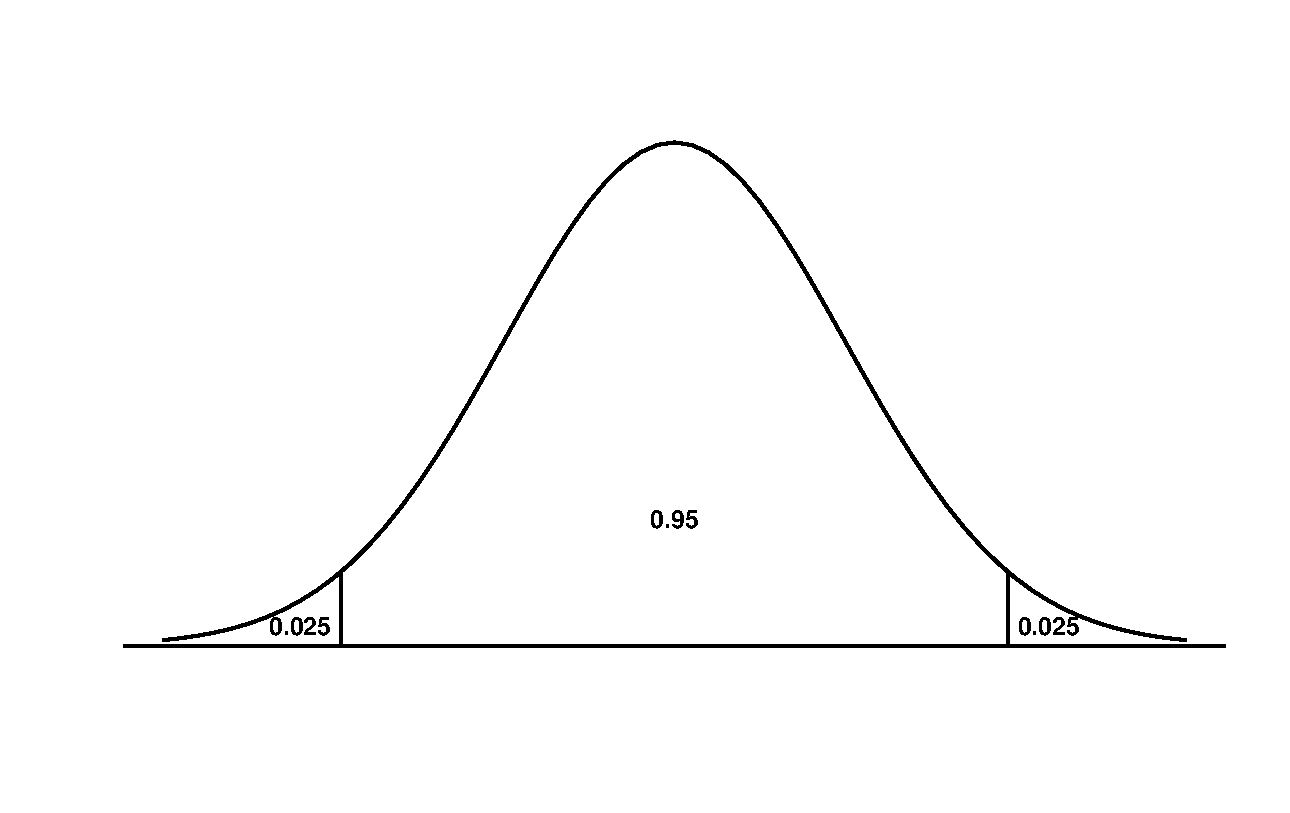
\includegraphics[width=2in]{zstar-eps-converted-to.pdf}}
    \begin{align*}
      P(-z^{*} \leq Z \leq z^{*}) = (1-\alpha)
      &\iff P( Z < -z^{*}) = \frac{\alpha}{2}
    \end{align*}
    \pause
    Thus, for a given confidence level $(1-\alpha)$, $z^*=z_{\alpha/2}$({\bf upper $\alpha/2$ critical point}), we can look up the
    corresponding $z^*$ value on the Normal table. \pause

\vspace{0.05cm}    
 {\bf Common $z^{*}$ values:}
    \begin{center}
      \begin{tabular}{c|ccc}
        Confidence Level& 90\% & 95\% & 99\% \\
        \hline
        $z^{*}$ & 1.645 & 1.96 & 2.576
      \end{tabular}
    \end{center}

\end{frame}
%%%%%%%%%%%%%%%%%%%%%%%%%%%%%%%%%%%%%%%%%%%%%%%%%%%%%%%%%%%%






\end{document}
